%!TeX encoding = UTF-8
%!TeX program = xelatex
\documentclass[notheorems, aspectratio=54]{beamer}
% aspectratio: 1610, 149, 54, 43(default), 32

\usepackage{latexsym}
\usepackage{amsmath,amssymb}
\usepackage{mathtools}
\usepackage{color,xcolor}
\usepackage{graphicx}
\usepackage{algorithm}
\usepackage{amsthm}
\DeclareMathOperator*{\argmax}{argmax} % thin space, limits underneath in displays
\usepackage{lmodern} % 解决 font warning
% \usepackage[UTF8]{ctex}
\usepackage{animate} % insert gif

\usepackage{lipsum} % To generate test text 
\usepackage{ulem} % 下划线,波浪线

\usepackage{listings} % display code on slides; don't forget [fragile] option after \begin{frame}

% ----------------------------------------------
% tikx
\usepackage{framed}
\usepackage{fancybox}
\usepackage{tikz}
\usepackage{tikz-qtree}
\usepackage{pgf}
\usetikzlibrary{automata, calc,trees,positioning,arrows,chains,shapes.geometric,%
    decorations.pathreplacing,decorations.pathmorphing,shapes,%
    matrix,shapes.symbols}
\pgfmathsetseed{1} % To have predictable results
% Define a background layer, in which the parchment shape is drawn
\pgfdeclarelayer{background}
\pgfsetlayers{background,main}

% define styles for the normal border and the torn border
\tikzset{
  normal border/.style={orange!30!black!10, decorate, 
     decoration={random steps, segment length=2.5cm, amplitude=.7mm}},
  torn border/.style={orange!30!black!5, decorate, 
     decoration={random steps, segment length=.5cm, amplitude=1.7mm}}}

% Macro to draw the shape behind the text, when it fits completly in the
% page
\def\parchmentframe#1{
\tikz{
  \node[inner sep=2em] (A) {#1};  % Draw the text of the node
  \begin{pgfonlayer}{background}  % Draw the shape behind
  \fill[normal border] 
        (A.south east) -- (A.south west) -- 
        (A.north west) -- (A.north east) -- cycle;
  \end{pgfonlayer}}}

% Macro to draw the shape, when the text will continue in next page
\def\parchmentframetop#1{
\tikz{
  \node[inner sep=2em] (A) {#1};    % Draw the text of the node
  \begin{pgfonlayer}{background}    
  \fill[normal border]              % Draw the ``complete shape'' behind
        (A.south east) -- (A.south west) -- 
        (A.north west) -- (A.north east) -- cycle;
  \fill[torn border]                % Add the torn lower border
        ($(A.south east)-(0,.2)$) -- ($(A.south west)-(0,.2)$) -- 
        ($(A.south west)+(0,.2)$) -- ($(A.south east)+(0,.2)$) -- cycle;
  \end{pgfonlayer}}}

% Macro to draw the shape, when the text continues from previous page
\def\parchmentframebottom#1{
\tikz{
  \node[inner sep=2em] (A) {#1};   % Draw the text of the node
  \begin{pgfonlayer}{background}   
  \fill[normal border]             % Draw the ``complete shape'' behind
        (A.south east) -- (A.south west) -- 
        (A.north west) -- (A.north east) -- cycle;
  \fill[torn border]               % Add the torn upper border
        ($(A.north east)-(0,.2)$) -- ($(A.north west)-(0,.2)$) -- 
        ($(A.north west)+(0,.2)$) -- ($(A.north east)+(0,.2)$) -- cycle;
  \end{pgfonlayer}}}

% Macro to draw the shape, when both the text continues from previous page
% and it will continue in next page
\def\parchmentframemiddle#1{
\tikz{
  \node[inner sep=2em] (A) {#1};   % Draw the text of the node
  \begin{pgfonlayer}{background}   
  \fill[normal border]             % Draw the ``complete shape'' behind
        (A.south east) -- (A.south west) -- 
        (A.north west) -- (A.north east) -- cycle;
  \fill[torn border]               % Add the torn lower border
        ($(A.south east)-(0,.2)$) -- ($(A.south west)-(0,.2)$) -- 
        ($(A.south west)+(0,.2)$) -- ($(A.south east)+(0,.2)$) -- cycle;
  \fill[torn border]               % Add the torn upper border
        ($(A.north east)-(0,.2)$) -- ($(A.north west)-(0,.2)$) -- 
        ($(A.north west)+(0,.2)$) -- ($(A.north east)+(0,.2)$) -- cycle;
  \end{pgfonlayer}}}

% Define the environment which puts the frame
% In this case, the environment also accepts an argument with an optional
% title (which defaults to ``Example'', which is typeset in a box overlaid
% on the top border
\newenvironment{parchment}[1][Example]{%
  \def\FrameCommand{\parchmentframe}%
  \def\FirstFrameCommand{\parchmentframetop}%
  \def\LastFrameCommand{\parchmentframebottom}%
  \def\MidFrameCommand{\parchmentframemiddle}%
  \vskip\baselineskip
  \MakeFramed {\FrameRestore}
  \noindent\tikz\node[inner sep=1ex, draw=black!20,fill=white, 
          anchor=west, overlay] at (0em, 2em) {\sffamily#1};\par}%
{\endMakeFramed}

% ----------------------------------------------

\mode<presentation>{
    \usetheme{CambridgeUS}
    % Boadilla CambridgeUS
    % default Antibes Berlin Copenhagen
    % Madrid Montpelier Ilmenau Malmoe
    % Berkeley Singapore Warsaw
    \usecolortheme{beaver}
    % beetle, beaver, orchid, whale, dolphin
    \useoutertheme{infolines}
    % infolines miniframes shadow sidebar smoothbars smoothtree split tree
    \useinnertheme{circles}
    % circles, rectanges, rounded, inmargin
}
% 设置 block 颜色
\setbeamercolor{block title}{bg=red!30,fg=white}

\newcommand{\reditem}[1]{\setbeamercolor{item}{fg=red}\item #1}

% 缩放公式大小
\newcommand*{\Scale}[2][4]{\scalebox{#1}{\ensuremath{#2}}}

% 解决 font warning
\renewcommand\textbullet{\ensuremath{\bullet}}

% ---------------------------------------------------------------------
% flow chart
\tikzset{
    >=stealth',
    punktchain/.style={
        rectangle, 
        rounded corners, 
        % fill=black!10,
        draw=white, very thick,
        text width=6em,
        minimum height=2em, 
        text centered, 
        on chain
    },
    largepunktchain/.style={
        rectangle,
        rounded corners,
        draw=white, very thick,
        text width=10em,
        minimum height=2em,
        on chain
    },
    line/.style={draw, thick, <-},
    element/.style={
        tape,
        top color=white,
        bottom color=blue!50!black!60!,
        minimum width=6em,
        draw=blue!40!black!90, very thick,
        text width=6em, 
        minimum height=2em, 
        text centered, 
        on chain
    },
    every join/.style={->, thick,shorten >=1pt},
    decoration={brace},
    tuborg/.style={decorate},
    tubnode/.style={midway, right=2pt},
    font={\fontsize{10pt}{12}\selectfont},
}
% ---------------------------------------------------------------------

% code setting
\lstset{
    language=C++,
    basicstyle=\ttfamily\footnotesize,
    keywordstyle=\color{red},
    breaklines=true,
    xleftmargin=2em,
    numbers=left,
    numberstyle=\color[RGB]{222,155,81},
    frame=leftline,
    tabsize=4,
    breakatwhitespace=false,
    showspaces=false,               
    showstringspaces=false,
    showtabs=false,
    morekeywords={Str, Num, List},
}

% ---------------------------------------------------------------------

%% preamble
\title{Lecture07}
% \subtitle{The subtitle}
\author{Dihui Lai}
\institute[WUSTL]{dlai@wustl.edu}

% -------------------------------------------------------------

\begin{document}

%% title frame
\begin{frame}
    \titlepage
\end{frame}



%% normal frame
\section{Neural Network}
\begin{frame}
    \center{Introduction to Neural Network}
\end{frame}
\begin{frame}
\frametitle{Neural Network: Topology}

\tikzset{%
  every neuron/.style={
    circle,
    draw,
    minimum size=0.8cm
  },
  neuron missing/.style={
    draw=none, 
    scale=2,
    text height=0.2cm,
    execute at begin node=\color{black}$\vdots$
  },
}

\begin{figure}
\centering
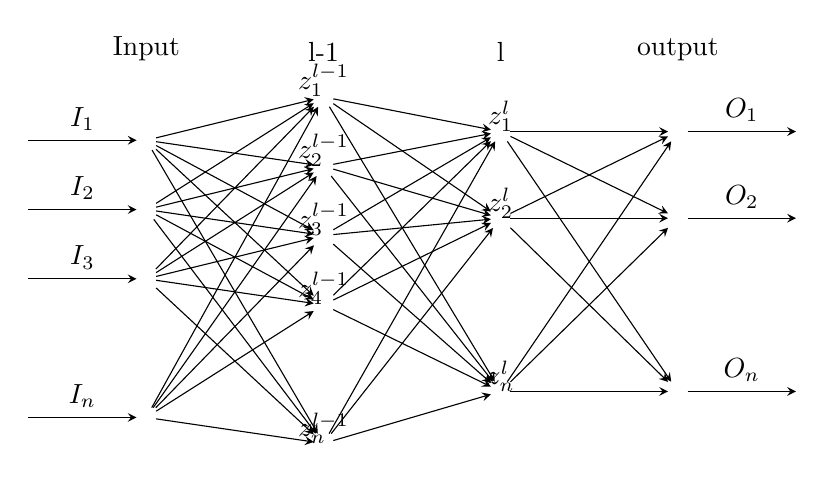
\begin{tikzpicture}[x=1.5cm, y=1.1cm, >=stealth]

\foreach \m/\l [count=\y] in {1,2,3,missing,4}
  \node [every neuron/.try, neuron \m/.try] (input-\m) at (0, 2-\y*0.8) {};

\foreach \m [count=\y] in {1, 2, 3, 4, missing, 5}
  \node [every neuron/.try, neuron \m/.try ] (hiddenl-\m) at (1.5, 2.5-\y*0.8) {};
  
\foreach \m [count=\y] in {1, 2, missing, 3}
  \node [every neuron/.try, neuron \m/.try ] (hidden-\m) at (3, 2.3-\y) {};
  
\foreach \m [count=\y] in {1,2, missing, 3}
  \node [every neuron/.try, neuron \m/.try ] (output-\m) at (4.5,2.3-\y) {};

\foreach \l [count=\i] in {1,2,3, n}
  \draw [<-] (input-\i) -- ++(-1,0)
    node [above, midway] {$I_\l$};

\foreach \l [count=\i] in {1, 2, 3, 4, n}
  \node [above] at (hiddenl-\i.south) {$z^{l-1}_\l$};

\foreach \l [count=\i] in {1, 2, n}
  \node [above] at (hidden-\i.south) {$z^{l}_\l$};
  
\foreach \l [count=\i] in {1,2, n}
  \draw [->] (output-\i) -- ++(1,0)
    node [above, midway] {$O_\l$};

\foreach \i in {1,...,4}
  \foreach \j in {1,...,5}
    \draw [->] (input-\i) -- (hiddenl-\j);
    
\foreach \i in {1,...,5}
  \foreach \j in {1,...,3}
    \draw [->] (hiddenl-\i) -- (hidden-\j);
    
\foreach \i in {1,...,3}
  \foreach \j in {1,...,3}
    \draw [->] (hidden-\i) -- (output-\j);

\foreach \l [count=\x from 0] in {Input, l-1, l, output}
  \node [align=center, above] at (\x*1.5,2) {\l};

\end{tikzpicture}
\end{figure}
\end{frame}

\begin{frame}
\frametitle{Neural Network: Forward}
    Each neuron at layer $\mathnormal{l}$ recieves inputs from all neuron from the previous layer $\mathnormal{l-1}$
    $$
    \mathnormal{z_k^l=\sum_jw^{l-1}_{kj}a_j^{l-1}}
    $$
  	The neuron tansfer the input signal $z_k^l$ via a transfer function $\sigma$ and send as input to to the next layer
    $$
	\mathnormal{a_k^l=\sigma(z_k^l)}
    $$
    The cost function of the neural network is dependeng on all the $z$s of neurons in all layers
    $$
    \mathnormal{C\left(z^l_1, z^l_2, ... z^l_k(z^{l-1}_1, z^{l-1}_2, z^{l-1}_3, ...), ...\right)}
    $$

\end{frame}

\begin{frame}
\frametitle{Neural Network: Activation Functions}
\begin{align*}
&\text{Step Function: } \mathnormal{\sigma (z)={\begin{cases}0&{\text{for }}z<0\\1&{\text{for }}z\geq 0\end{cases}}}\\
&\text{Logistic/Sigmoid: } \mathnormal{\sigma (z)={\frac {1}{1+e^{-z}}}}\\
&\text{hyperbolic tangent: }  \mathnormal{\sigma(z)={\frac {(e^{z}-e^{-z})}{(e^{z}+e^{-z})}}}\\
&\text{ReLU: } \mathnormal{\sigma(z)={\begin{cases}0&{\text{for }}z\leq 0\\z&{\text{for }}z>0\end{cases}}}
\end{align*}
Reference \url{https://en.wikipedia.org/wiki/Activation_function}
\end{frame}



\begin{frame}
\frametitle{Optimization: Stochastic Gradient Descent Method}
\begin{enumerate}
\item Update the weights by changing it along the gradient to reduce the cost function
\item do one data point at a time
\end{enumerate}
$$\mathnormal{w_j \leftarrow w_j-\eta \frac{\partial C^i(w_j)}{\partial w_j}}, i =1, 2, 3, ...n$$
\end{frame}



\begin{frame}

\frametitle{Gradient Descent Method for Linear Regression}
Cost function $\mathnormal{C(\beta)=\sum_i\frac{1}{2}(y^i-\vec{x}^i\cdot\vec{\beta})^2}$

$$\mathnormal{\frac{\partial C}{\partial \beta_j}=\sum_j(\hat{y}^i-y^i)x_j^i}$$

The corresponding stochastic gradient methods is 
$$\mathnormal{\beta_j\leftarrow \beta_j+\epsilon(y^i-\hat{y}^i)x_j^i}$$

The update method is quite intuitive considering that $\mathnormal{\beta_j}$ is adjusted higher if estimated $\mathnormal{\hat{y}^i}$ is less than $\mathnormal{y^i}$; adjusted lower if $\mathnormal{\hat{y}^i}$ is more than $\mathnormal{y^i}$

\end{frame}	

\begin{frame}

\frametitle{mini-Batch Gradient Descent}

Between use the full data set or use 1 single data point to update $\mathnormal{ w}$, one can choose to update $\mathnormal{w}$ by calculating gradient using $\mathnormal{m}$ data points or called a mini-batch. 

Dividing the data set to $\mathnormal{k}$ mini-batch so that $\mathnormal{km=n}$. Iterating through $\mathnormal{k}$ mini-batches is called an epoch

\end{frame}	

\begin{frame}
\frametitle{Neural Network: Backpropogation}

\tikzset{%
  every neuron/.style={
    circle,
    draw,
    minimum size=1cm
  },
  neuron missing/.style={
    draw=none, 
    scale=1,
    text height=0.333cm,
    execute at begin node=\color{black}$\vdots$
  },
}

\begin{figure}
\centering
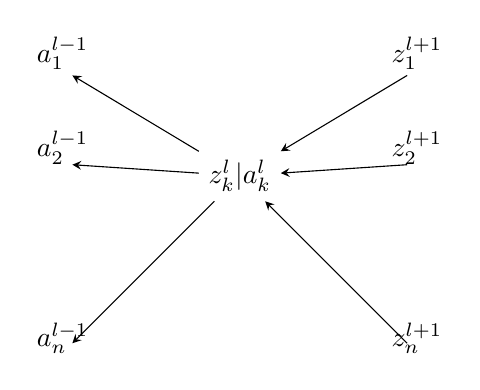
\begin{tikzpicture}[x=1.5cm, y=1.5cm, >=stealth]
\foreach \m [count=\y] in {1, 2, missing, 3}
  \node [every neuron/.try, neuron \m/.try ] (hiddenl-\m) at (2, 2.5-\y*0.8) {};
  
\foreach \m [count=\y] in {2}
  \node [every neuron/.try, neuron \m/.try ] (hidden-\m) at (3.5, 1.8-\y) {$z^{l}_k|a_k^{l}$};
  
\foreach \m [count=\y] in {1,2, missing, 3}
  \node [every neuron/.try, neuron \m/.try ] (output-\m) at (5, 2.5-\y*0.8) {};

\foreach \l [count=\i] in {1, 2, n}
  \node [above] at (hiddenl-\i.south) {$a^{l-1}_{\l}$};
  
\foreach \l [count=\i] in {1, 2, n}
  \node [above] at (output-\i.south) {$z^{l+1}_{\l}$};
  
\foreach \i in {1,...,3}
  \foreach \j in {2}
    \draw [<-] (hiddenl-\i) -- (hidden-\j);

\foreach \i in {2}
  \foreach \j in {1,...,3}
    \draw [<-] (hidden-\i) -- (output-\j);
\end{tikzpicture}
\end{figure}


\end{frame}
\begin{frame}

\frametitle{Neural Network: Backpropogation}
The contribution to the cost function from a neuron in layer $l$ can be cauculated iteratively as
\begin{align*}
\mathnormal{\delta^l_k=\frac{\partial C}{\partial z_k^l}}&=\mathnormal{\sum_m \frac{\partial C}{\partial z_m^{l+1}}\frac{\partial z_m^{l+1}}{\partial z_k^l}}\\
&=\mathnormal{\left(\sum_m \frac{\partial C}{\partial z_m^{l+1}}\frac{\partial z_m^{l+1}}{\partial a_k^l}\right)\frac{\partial a_k^l}{\partial z_k^l}}\\
&=\mathnormal{\sum_m \delta^{l+1}_m w^l_{mk}\sigma'(z_k^l)}
\end{align*}
The partial derivative of a cost function w.r.t the weight $\mathnormal{w_{kj}^{l-1}}$ is 
$$
\mathnormal{\frac{\partial C}{\partial w_{kj}^{l-1}}=\frac{\partial C}{\partial z_k^l}\frac{\partial z_k^l}{\partial w_{kj}^{l-1}}=\delta^l_k a^{l-1}_j}
$$
\end{frame}

\begin{frame}
\frametitle{Training Neural Network}
\begin{enumerate}
\item Define the topology of your neural network: number of layers, number of units in each layer
\item initialize the weights $\mathnormal{w}$ of the network
\item calculate the gradient of cost function by calculating $\delta^k_l$ against all neurons, backpropogate iteratively 
\item updates weights of the network along with the gradient
\begin{itemize}
\item batch gradient descent
\item mini-batch gradient descent
\item stochastic gradient descent
\end{itemize}
\end{enumerate}
\end{frame}



\begin{frame}
\frametitle{Multinomial distribution and multi-class classification}

Multinomial distribution: there could be $\mathnormal{c}$ outcome of an experiment, each of probability  $\mathnormal{p_1}$, $\mathnormal{p_2}$, $\mathnormal{p_3}$, ..., $\mathnormal{p_c}$ and $\mathnormal{\sum\limits_{j=1}^c p_j=1}$. If one perform $\mathnormal{N}$ experiments, the probability of getting $\mathnormal{x_1}$, $\mathnormal{x_2}$, $\mathnormal{x_3}$, ... $\mathnormal{x_c}$ of each out come can be described as 
$$\mathnormal{f(x_1, x_2, x_3, ... x_c)=\frac{N!}{x_1! x_2! ... x_c!} p_1^{x_1} p_2^{x_2} ... p_c^{x_c}}$$

The likelihood function can be accordingly written as 
$\mathnormal{L= \prod \limits_{i=1}^n\prod \limits_{j=1}^c p_{j}^{x^i_j}}$

The log-likelihood function (a.k.a log-loss) is
$$\mathnormal{\ell=\log(L)=\sum\limits_{i=1}^n \sum\limits_{j=1}^c x_j^i \log(p_j)}$$
\end{frame}

\end{document}

